\documentclass[10pt]{beamer}
\usetheme[
%%% options passed to the outer theme
%    hidetitle,           % hide the (short) title in the sidebar
%    hideauthor,          % hide the (short) author in the sidebar
%    hideinstitute,       % hide the (short) institute in the bottom of the sidebar
%    shownavsym,          % show the navigation symbols
%    width=2cm,           % width of the sidebar (default is 2 cm)
%    hideothersubsections,% hide all subsections but the subsections in the current section
%    hideallsubsections,  % hide all subsections
    right               % right of left position of sidebar (default is right)
%%% options passed to the color theme
%    lightheaderbg,       % use a light header background
  ]{AAUsidebar}

% If you want to change the colors of the various elements in the theme, edit and uncomment the following lines
% Change the bar and sidebar colors:
%\setbeamercolor{AAUsidebar}{fg=red!20,bg=red}
%\setbeamercolor{sidebar}{bg=red!20}
% Change the color of the structural elements:
%\setbeamercolor{structure}{fg=red}
% Change the frame title text color:
%\setbeamercolor{frametitle}{fg=blue}
% Change the normal text color background:
%\setbeamercolor{normal text}{bg=gray!10}
% ... and you can of course change a lot more - see the beamer user manual.


\usepackage[utf8]{inputenc}
\usepackage[english]{babel}
\usepackage[T1]{fontenc}
% Or whatever. Note that the encoding and the font should match. If T1
% does not look nice, try deleting the line with the fontenc.
\usepackage{helvet}

% colored hyperlinks
\newcommand{\chref}[2]{%
  \href{#1}{{\usebeamercolor[bg]{AAUsidebar}#2}}%
}

\title[IoTsec: Automatic Profile-based Firewall for IoT Devices]% optional, use only with long paper titles
{IoTsec}

\subtitle{Automatic Profile-based Firewall for IoT Devices}  % could also be a conference name

\date{21. June 2017}

\author[] % optional, use only with lots of authors
{
  Daniel Amkær Sørensen \\ \& \\ Nichlas Vanggaard
}
% - Give the names in the same order as they appear in the paper.
% - Use the \inst{?} command only if the authors have different
%   affiliation. See the beamer manual for an example

\institute[
%  {\includegraphics[scale=0.2]{aau_segl}}\\ %insert a company, department or university logo
  Networks and Distributed Systems\\
  Aalborg University\\
  Denmark\\
] % optional - is placed in the bottom of the sidebar on every slide
{% is placed on the title page
  Networks and Distributed Systems\\
  Aalborg University\\
  Denmark\\
  
  %there must be an empty line above this line - otherwise some unwanted space is added between the university and the country (I do not know why;( )
}


% specify a logo on the titlepage (you can specify additional logos an include them in 
% institute command below
\pgfdeclareimage[height=1.5cm]{titlepagelogo}{AAUgraphics/aau_logo_new} % placed on the title page
%\pgfdeclareimage[height=1.5cm]{titlepagelogo2}{graphics/aau_logo_new} % placed on the title page
\titlegraphic{% is placed on the bottom of the title page
  \pgfuseimage{titlepagelogo}
%  \hspace{1cm}\pgfuseimage{titlepagelogo2}
}


\begin{document}
% the titlepage
{\aauwavesbg%
\begin{frame}[plain,noframenumbering] % the plain option removes the sidebar and header from the title page
  \titlepage
\end{frame}}
%%%%%%%%%%%%%%%%

% TOC
\begin{frame}{Agenda}{}
\tableofcontents
\end{frame}
%%%%%%%%%%%%%%%%

%%%%%%%%%%
% Inputs %
%%%%%%%%%%


\newpage
\section{Motivation}
\begin{frame}{Motivation}{Mirai}


\begin{minipage}{0.48\textwidth}
\begin{itemize}
	\item 21. October 2016
	\item Dyn attack 
	\begin{itemize}
		\item Netflix
		\item Twitter
		\item Spotify
		\item Reddit
	\end{itemize}
	\item 620 Gbps
	\item 100.000 - 500.000 devices
	\item Default credentials
	\item Amnesia
	
\end{itemize}
\end{minipage}
\hfill
\begin{minipage}{0.48\textwidth}
\vspace{0.4\textheight}
	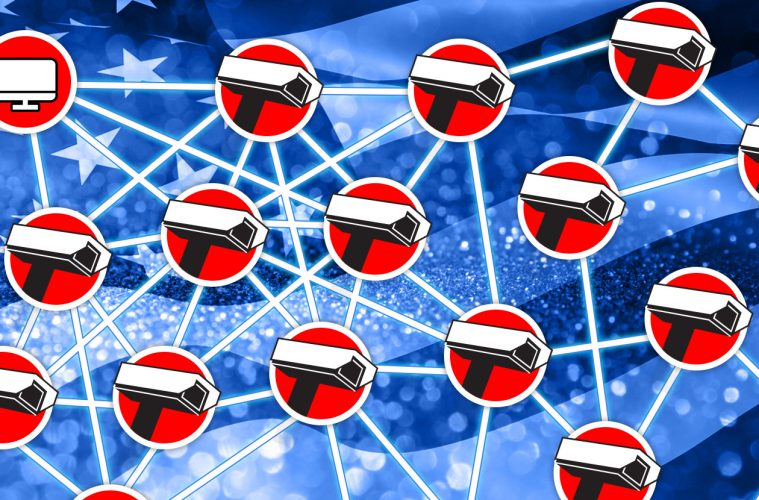
\includegraphics[width=\textwidth]{figs/botnet}
\end{minipage}
\end{frame}

\section{Report: F-Secure}

\begin{frame}{New Report from F-Secure}
\begin{minipage}{0.48\textwidth}
\begin{itemize}
	\item Foscam 
	\item 18 vulnerabilities
	\begin{itemize}
		\item Default credentials
		\item Hardcoded credentials
		\item Hidden services
		\item etc.
	\end{itemize}
	\item White label
	\begin{itemize}
		\item At least 14 brands
	\end{itemize}
\end{itemize}

\end{minipage}
%
\hfill
%
\begin{minipage}{0.48\textwidth}
\begin{figure}
	
	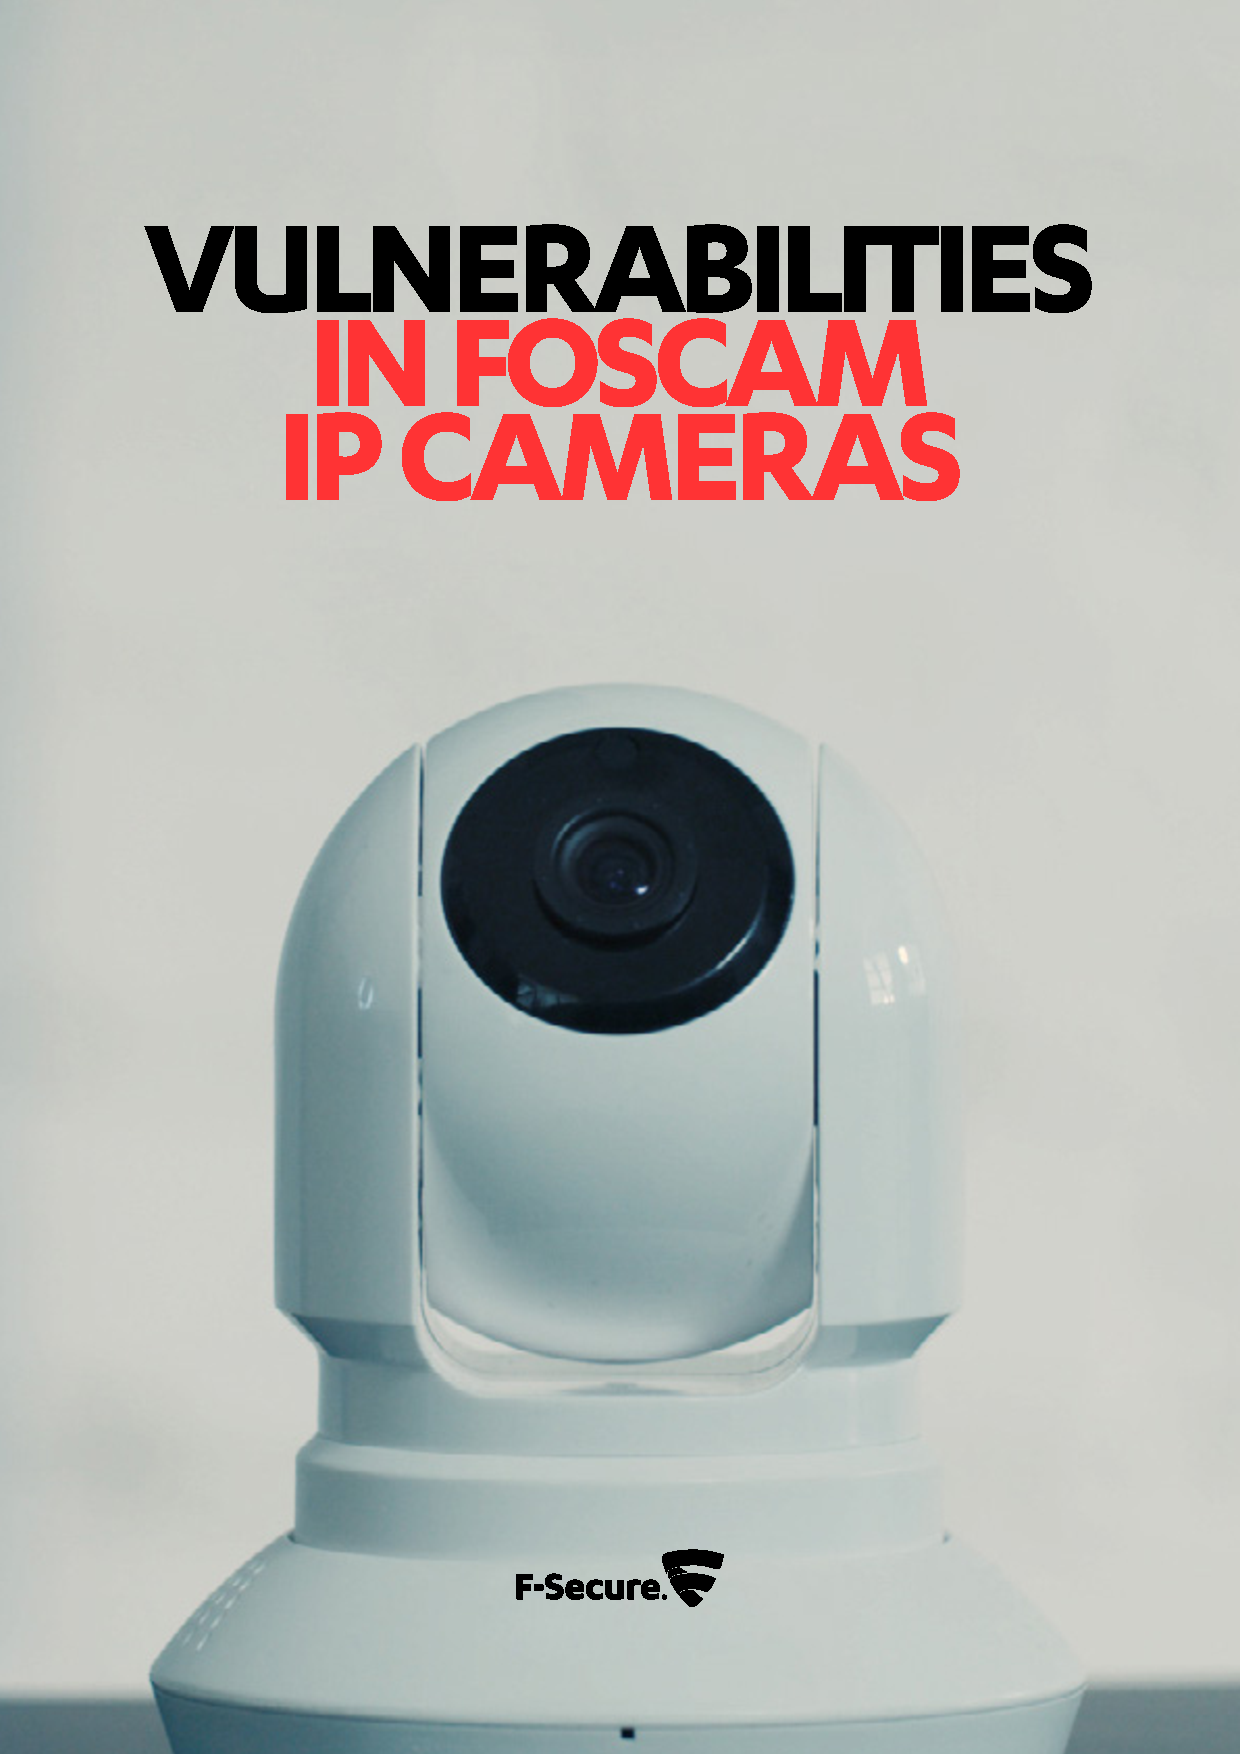
\includegraphics[width=\textwidth]{figs/f-secure}
\end{figure}
\end{minipage}

\end{frame}

\subsection{Recommendations}
\begin{frame}{F-secure Recommendations}

\begin{itemize}
	\item Users
\begin{itemize}
	\item IoT devices on seperate network / VLAN
	\item Always change credentials
\end{itemize}
	\item Corporate
\begin{itemize}
	\item Never assume anything to be secure without evidence
	\item Do security testing before deployment
\end{itemize}
	\item Vendors
\begin{itemize}
	\item Make existing fixes available for all models in a coordinated way
	\item Never trust user input
	\item Remove unused services
	\item Avoid hardcoded credentials
\end{itemize}
\end{itemize}
	
\end{frame}

\begin{frame}{Vendor Response}
\begin{itemize}
	\item Foscam has not responded to F-secure
	\item White label products seem more vulnerable
	\begin{itemize}
		\item Foscam cameras
		\item DVRs targeted by Amnesia
	\end{itemize}
	\item ``Secure'' devices
	\begin{itemize}
		\item Tado
		\item Philips Hue
	\end{itemize}
\end{itemize}

\end{frame}


\end{document}
